% Für Bindekorrektur als optionales Argument "BCORfaktormitmaßeinheit", dann
% sieht auch Option "twoside" vernünftig aus
% Näheres zu "scrartcl" bzw. "scrreprt" und "scrbook" siehe KOMA-Skript Doku
\documentclass[12pt,a4paper,titlepage,headinclude,bibtotoc]{scrartcl}


%---- Allgemeine Layout Einstellungen ------------------------------------------

% Für Kopf und Fußzeilen, siehe auch KOMA-Skript Doku
\usepackage[komastyle]{scrpage2}
\pagestyle{scrheadings}
\setheadsepline{0.5pt}[\color{black}]
\automark[section]{chapter}


%Einstellungen für Figuren- und Tabellenbeschriftungen
\setkomafont{captionlabel}{\sffamily\bfseries}
\setcapindent{0em}


%---- Weitere Pakete -----------------------------------------------------------
% Die Pakete sind alle in der TeX Live Distribution enthalten. Wichtige Adressen
% www.ctan.org, www.dante.de

% Sprachunterstützung
\usepackage[ngerman]{babel}

% Benutzung von Umlauten direkt im Text
% entweder "latin1" oder "utf8"
\usepackage[utf8]{inputenc}

% Pakete mit Mathesymbolen und zur Beseitigung von Schwächen der Mathe-Umgebung
\usepackage{latexsym,exscale,stmaryrd,amssymb,amsmath}

% Weitere Symbole
\usepackage[nointegrals]{wasysym}
\usepackage{eurosym}

% Anderes Literaturverzeichnisformat
%\usepackage[square,sort&compress]{natbib}

% Für Farbe
\usepackage{color}

% Zur Graphikausgabe
%Beipiel: \includegraphics[width=\textwidth]{grafik.png}
\usepackage{graphicx}

% Text umfließt Graphiken und Tabellen
% Beispiel:
% \begin{wrapfigure}[Zeilenanzahl]{"l" oder "r"}{breite}
%   \centering
%   \includegraphics[width=...]{grafik}
%   \caption{Beschriftung} 
%   \label{fig:grafik}
% \end{wrapfigure}
\usepackage{wrapfig}

% Mehrere Abbildungen nebeneinander
% Beispiel:
% \begin{figure}[htb]
%   \centering
%   \subfigure[Beschriftung 1\label{fig:label1}]
%   {\includegraphics[width=0.49\textwidth]{grafik1}}
%   \hfill
%   \subfigure[Beschriftung 2\label{fig:label2}]
%   {\includegraphics[width=0.49\textwidth]{grafik2}}
%   \caption{Beschriftung allgemein}
%   \label{fig:label-gesamt}
% \end{figure}
\usepackage{subfigure}
\usepackage{adjustbox}
%\begin{figure}[h]
%  \centering
%  \subfigure[Caption1\label{fig:bild1}]
%  {\begin{adjustbox}{width=0.44\linewidth}\input{bild1}\end{adjustbox}}
%  \hfill
%  \subfigure[Caption2\label{bild2}]
%  {\begin{adjustbox}{width=0.44\linewidth}\input{bild2}\end{adjustbox}}
%  \hfill
%  \subfigure[Caption3\label{bild3}]
%  {\begin{adjustbox}{width=0.44\linewidth}\input{bild3}\end{adjustbox}}
%  \caption{$u$ und $v$ gegen $t$ und $u$ gegen $v$ aufgetragen für $b=0.4$}
%  \label{fig:gesamtlabel}
%\end{figure}


% Caption neben Abbildung
% Beispiel:
% \sidecaptionvpos{figure}{"c" oder "t" oder "b"}
% \begin{SCfigure}[rel. Breite (normalerweise = 1)][hbt]
%   \centering
%   \includegraphics[width=0.5\textwidth]{grafik.png}
%   \caption{Beschreibung}
%   \label{fig:}
% \end{SCfigure}
\usepackage{sidecap}

% Befehl für "Entspricht"-Zeichen
\newcommand{\corresponds}{\ensuremath{\mathrel{\widehat{=}}}}
% Befehl für Errorfunction
\newcommand{\erf}[1]{\text{ erf}\ensuremath{\left( #1 \right)}}

%Fußnoten zwingend auf diese Seite setzen
\interfootnotelinepenalty=1000

%Für chemische Formeln (von www.dante.de)
%% Anpassung an LaTeX(2e) von Bernd Raichle
\makeatletter
\DeclareRobustCommand{\chemical}[1]{%
  {\(\m@th
   \edef\resetfontdimens{\noexpand\)%
       \fontdimen16\textfont2=\the\fontdimen16\textfont2
       \fontdimen17\textfont2=\the\fontdimen17\textfont2\relax}%
   \fontdimen16\textfont2=2.7pt \fontdimen17\textfont2=2.7pt
   \mathrm{#1}%
   \resetfontdimens}}
\makeatother

%Honecker-Kasten mit $$\shadowbox{$xxxx$}$$
\usepackage{fancybox}

%SI-Package
\usepackage{siunitx}

%keine Einrückung, wenn Latex doppelte Leerzeile
\parindent0pt

%Bibliography \bibliography{literatur} und \cite{gerthsen}
%\usepackage{cite}
\usepackage{babelbib}
\selectbiblanguage{ngerman}

\begin{document}

\begin{titlepage}
\centering
\textsc{\Large Anfängerpraktikum der Fakultät für
  Physik,\\[1.5ex] Universität Göttingen}

\vspace*{3cm}

\rule{\textwidth}{1pt}\\[0.5cm]
{\huge \bfseries
  Versuch Kennlinien der Vakuum-Diode\\[1.5ex]
  Protokoll}\\[0.5cm]
\rule{\textwidth}{1pt}

\vspace*{3cm}

\begin{Large}
\begin{tabular}{ll}
Praktikant: &  Michael Lohmann\\
 &  Felix Kurtz\\
% &  Kevin Lüdemann\\
% &  Skrollan Detzler\\
 E-Mail: & m.lohmann@stud.uni-goettingen.de\\
 &  felix.kurtz@stud.uni-goettingen.de\\
% &  kevin.luedemann@stud.uni-goettingen.de\\
% &  skrollan.detzler@stud.uni-goettingen.de\\
 Betreuer: &Björn Klaas\\
 Versuchsdatum: & 12.09.2014\\
\end{tabular}
\end{Large}

\vspace*{0.8cm}

\begin{Large}
\fbox{
  \begin{minipage}[t][2.5cm][t]{6cm} 
    Testat:
  \end{minipage}
}
\end{Large}

\end{titlepage}

\tableofcontents

\newpage

\section{Einleitung}
\label{sec:einleitung}
Dioden sind technische Bauelemente, die nur einen Stromfluss in eine Richtung zulassen.
Vakuum-Dioden sind die wohl einfachsten, wenn auch heutzutage nicht mehr die gebräuchlichsten.
Ihre wichtigsten Kennlinien zu vermessen, kann daher Erkenntnisse für komplexere Aufbauten, wie zum Beispiel Halbleiterdioden, liefern.


\section{Theorie}
\label{sec:theorie}
\subsection{Austrittsarbeit der Elektronen}
Eine Vakuum-Diode besteht aus einem Kathode-Anode-Paar, welches in einem Vakuum-Behältnis eingelassen ist.
Die Kathode besteht aus einer Glühlampe, welche regelbar beheizt werden kann.
Die Elektronen benötigen eine gewisse Energie $W_A$ um aus dem Draht auszutreten und zur Anode zu gelangen.
Sie wird dafür benötigt, sich aus dem positiv geladenen Gitter des Drahtes herauszulösen.
Diese Energie ist jedoch relativ hoch, so dass bei den hier verwendeten Spannungen kein Strom zu messen sein sollte.
Da die Kathode jedoch auf eine Temperatur $T$ geheizt wird, bekommen die Elektronen im Draht eine thermische (und damit kinetische) Energie.
Dies ist auch der Grund, warum die Vakuum-Diode einen Elektronenfluss von der Anode zur Kathode verhindert.
Nicht alle Elektronen sind jedoch gleich schnell, so dass einige mehr kinetische besitzen als andere.
Die Verteilung der Geschwindigkeiten basiert auf der \textsc{Fermi}-Verteilung.
Der sich so ergebende Strom verhält sich nach der \textsc{Richardson}\emph{-Gleichung}:
\begin{align}
	j_R=A_R\cdot T^{2}\cdot \exp\left(-\frac{W_A}{k_BT}\right)\label{eq:richardson}\; .
\end{align}
Wobei $A_R\approx \SI{6e-3}{\ampere\meter^{-2}\kelvin^{-2}}$ die Richardson-Konstante darstellt.
Sie ist für alle reinen Metalle etwa gleich.
Zur Verringerung der Austrittsarbeit $W_A$ können Metalle mit Alkalimetallen oder Barium-Oxid überzogen werden, da diese eine geringere besitzen.


                                                                                                                                                                      
\subsection{Vakuumdiode}
Eine Vakuumdiode besteht aus einer Anode und einer beheizbaren Kathode, welche zusammen in einem evakuierten Glaskolben eingeschlossen sind.
Zwischen ihnen können Elektronen von der Kathode aus sich bewegen, wenn die Heizspannung hoch genug ist.
Dies liegt daran, dass die Elektronen durch die bloße Anodenspannung nicht genügend Energie besitzen, um die Austrittsarbeit zu überwinden.
Wird der Draht beheizt, so bekommen die Elektronen dadurch eine höhere kinetische Energie.
Die mittlere kinetische Energie reicht zwar immer noch nicht, um den Draht zu verlassen.
Aber da die Energien \textsc{Maxwell}-verteilt sind, haben einzelne Elektronen auch bei geringeren Temperaturen eine genügend hohe Energie.\\
\begin{figure}[!h]
\centering
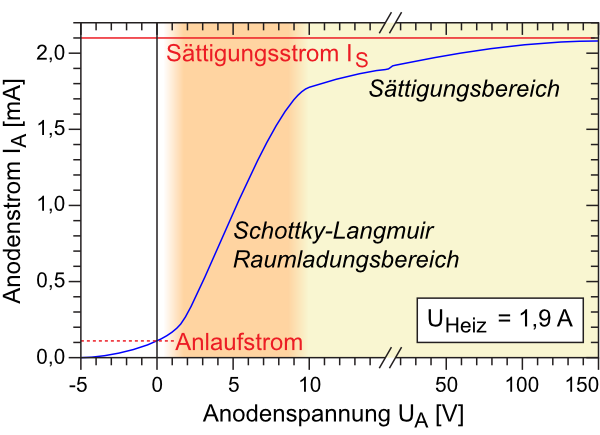
\includegraphics{stromfluss}
\caption{Stromfluss gegen die Anodenspannung aufgetragen von \cite[8.10.14, 12 Uhr]{LP17}}
\label{fig:strombild}
\end{figure}

Die folgenden Bereiche beziehen sich auf Abb. \ref{fig:strombild}.

Der \textbf{Anlaufstrom} ist der Strom, der fließt, ohne, dass eine Spannung zwischen den Elektroden anliegt.
Dieser ist nicht verschwindend, da aus der Kathode gelöste Elektronen durch Zufall auf die Anode auftreffen können.

Der \textbf{Raumladungsbereich} ist der Bereich in der Anodenspannung, in dem der Anodenstrom ungefähr linear ansteigt.
Dies geschieht dadurch, dass genügend Elektronen aus der Kathode durch die thermische Energie herausgelöst werden.
Es können sich aber nicht alle herausgelösten Elektronen zur Anode bewegen, da Elektronen, die schon auf dem Weg sind, das elektrische Feld abschirmen.
Hier gilt nach \cite[S. 475]{gerthsen} das \textsc{Schoty-Lamour}sche Raumladungsgesetz:
\begin{align}
j=\frac{4}{9}\varepsilon_0\cdot\sqrt\frac{2e}{m_e}\frac{U^{3/2}}{d^2}\, .\label{eq:rauml}
\end{align}

Wird die \textbf{Anodenspannung} jedoch immer größer, so ist irgendwann ein Sättigungsbereich erreicht.
In diesem sind keine Elektronen mehr im Raumladungsbereich vorhanden und um einen höheren Anodenstrom zu erziehlen, muss die Anodenspannung sehr viel größer werden.



\section{Durchführung}
\label{sec:durchfuehrung}
\begin{figure}[!h]
\centering
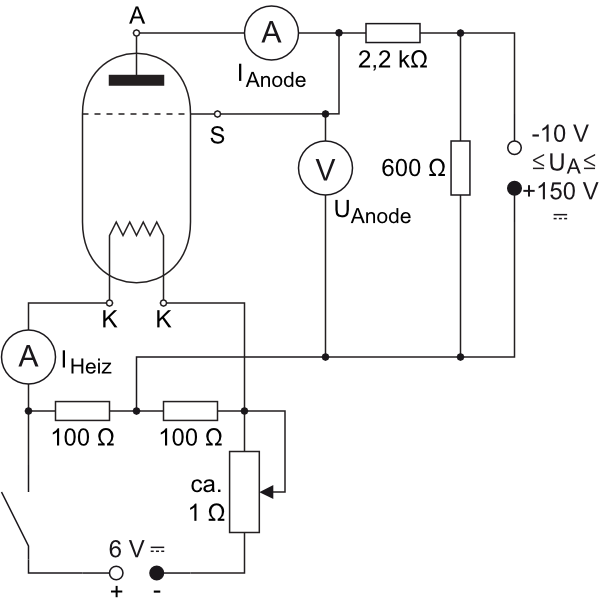
\includegraphics[width=0.5\linewidth]{aufbau}
\caption{Schaltplan der Vakuumdiode aus \cite[8.10.14, 12 Uhr]{LP17}}
\label{fig:aufbau}
\end{figure}
Zunächst baut man die Schaltung aus Abb. \ref{fig:aufbau} auf.
Dabei ist darauf zu achten, dass die Schutzringe zwar auf dem Anodenpotential sind, aber der darüber fließende Strom nicht fälschlicher weise als Anodenstrom gmessen wird.\\
Dann wählt man drei verschiedene Heizströme zwischen 1.8 A und 2 A und zeichnet für sie jeweils zu unterschiedlichen Anodenspannungen zwischen $-10\,$V und $150\,$V die zugehörigen Anodenströme auf.
Im Bereich des Anlaufstroms und der Raumladung sollten die Messungen in höchstens 2 V-Schritten erfolgen.
Die Spannung soll soweit heruntergeregelt werden, bis kein Anodenstrom mehr messbar ist.
Auch der Bereich um $U_A=0\,$V soll sehr genau vermessen werden.

\section{Auswertung}
\label{sec:auswertung}
\subsection{Kennlinien}
In Abb. \ref{fig:heiz} werden für verschiedene Heizströme die gemessenen Anodenströme aufgetragen.
Die Achsen sind für die einzelnen Plots bewusst anders skaliert.
Die Grafik \ref{fig:h} zeigt alle Messungen zusammen.
Dabei kann man klar erkennen, dass mit steigendem Heizstrom auch ein deutlich höherer Anodenstrom fließen kann.
Für die Fehler der Anodenspannungsmessung wurde $\sigma_{U_A}=U_A\cdot 0.25\%+1$ Digit verwendet.
Der Strommessung des Anodenstroms wurde eine Ungenauigkeit von $\sigma_{I_A}= I_A\cdot 0.8\%+2$ Digits zugewiesen.
\begin{figure}[h]
  \centering
  \subfigure[$I_\text H=1.8\,$A\label{fig:heiz18}]
  {\begin{adjustbox}{width=0.48\linewidth}% GNUPLOT: LaTeX picture with Postscript
\begingroup
  \makeatletter
  \providecommand\color[2][]{%
    \GenericError{(gnuplot) \space\space\space\@spaces}{%
      Package color not loaded in conjunction with
      terminal option `colourtext'%
    }{See the gnuplot documentation for explanation.%
    }{Either use 'blacktext' in gnuplot or load the package
      color.sty in LaTeX.}%
    \renewcommand\color[2][]{}%
  }%
  \providecommand\includegraphics[2][]{%
    \GenericError{(gnuplot) \space\space\space\@spaces}{%
      Package graphicx or graphics not loaded%
    }{See the gnuplot documentation for explanation.%
    }{The gnuplot epslatex terminal needs graphicx.sty or graphics.sty.}%
    \renewcommand\includegraphics[2][]{}%
  }%
  \providecommand\rotatebox[2]{#2}%
  \@ifundefined{ifGPcolor}{%
    \newif\ifGPcolor
    \GPcolortrue
  }{}%
  \@ifundefined{ifGPblacktext}{%
    \newif\ifGPblacktext
    \GPblacktexttrue
  }{}%
  % define a \g@addto@macro without @ in the name:
  \let\gplgaddtomacro\g@addto@macro
  % define empty templates for all commands taking text:
  \gdef\gplbacktext{}%
  \gdef\gplfronttext{}%
  \makeatother
  \ifGPblacktext
    % no textcolor at all
    \def\colorrgb#1{}%
    \def\colorgray#1{}%
  \else
    % gray or color?
    \ifGPcolor
      \def\colorrgb#1{\color[rgb]{#1}}%
      \def\colorgray#1{\color[gray]{#1}}%
      \expandafter\def\csname LTw\endcsname{\color{white}}%
      \expandafter\def\csname LTb\endcsname{\color{black}}%
      \expandafter\def\csname LTa\endcsname{\color{black}}%
      \expandafter\def\csname LT0\endcsname{\color[rgb]{1,0,0}}%
      \expandafter\def\csname LT1\endcsname{\color[rgb]{0,1,0}}%
      \expandafter\def\csname LT2\endcsname{\color[rgb]{0,0,1}}%
      \expandafter\def\csname LT3\endcsname{\color[rgb]{1,0,1}}%
      \expandafter\def\csname LT4\endcsname{\color[rgb]{0,1,1}}%
      \expandafter\def\csname LT5\endcsname{\color[rgb]{1,1,0}}%
      \expandafter\def\csname LT6\endcsname{\color[rgb]{0,0,0}}%
      \expandafter\def\csname LT7\endcsname{\color[rgb]{1,0.3,0}}%
      \expandafter\def\csname LT8\endcsname{\color[rgb]{0.5,0.5,0.5}}%
    \else
      % gray
      \def\colorrgb#1{\color{black}}%
      \def\colorgray#1{\color[gray]{#1}}%
      \expandafter\def\csname LTw\endcsname{\color{white}}%
      \expandafter\def\csname LTb\endcsname{\color{black}}%
      \expandafter\def\csname LTa\endcsname{\color{black}}%
      \expandafter\def\csname LT0\endcsname{\color{black}}%
      \expandafter\def\csname LT1\endcsname{\color{black}}%
      \expandafter\def\csname LT2\endcsname{\color{black}}%
      \expandafter\def\csname LT3\endcsname{\color{black}}%
      \expandafter\def\csname LT4\endcsname{\color{black}}%
      \expandafter\def\csname LT5\endcsname{\color{black}}%
      \expandafter\def\csname LT6\endcsname{\color{black}}%
      \expandafter\def\csname LT7\endcsname{\color{black}}%
      \expandafter\def\csname LT8\endcsname{\color{black}}%
    \fi
  \fi
  \setlength{\unitlength}{0.0500bp}%
  \begin{picture}(7200.00,5040.00)%
    \gplgaddtomacro\gplbacktext{%
      \csname LTb\endcsname%
      \put(946,704){\makebox(0,0)[r]{\strut{} 0}}%
      \put(946,1383){\makebox(0,0)[r]{\strut{} 0.2}}%
      \put(946,2061){\makebox(0,0)[r]{\strut{} 0.4}}%
      \put(946,2740){\makebox(0,0)[r]{\strut{} 0.6}}%
      \put(946,3418){\makebox(0,0)[r]{\strut{} 0.8}}%
      \put(946,4097){\makebox(0,0)[r]{\strut{} 1}}%
      \put(946,4775){\makebox(0,0)[r]{\strut{} 1.2}}%
      \put(1078,484){\makebox(0,0){\strut{}-20}}%
      \put(1714,484){\makebox(0,0){\strut{} 0}}%
      \put(2350,484){\makebox(0,0){\strut{} 20}}%
      \put(2986,484){\makebox(0,0){\strut{} 40}}%
      \put(3622,484){\makebox(0,0){\strut{} 60}}%
      \put(4259,484){\makebox(0,0){\strut{} 80}}%
      \put(4895,484){\makebox(0,0){\strut{} 100}}%
      \put(5531,484){\makebox(0,0){\strut{} 120}}%
      \put(6167,484){\makebox(0,0){\strut{} 140}}%
      \put(6803,484){\makebox(0,0){\strut{} 160}}%
      \put(176,2739){\rotatebox{-270}{\makebox(0,0){\strut{}Anodenstrom $I_\text A \; [A]$}}}%
      \put(3940,154){\makebox(0,0){\strut{}Spannung U $[V]$}}%
    }%
    \gplgaddtomacro\gplfronttext{%
      \csname LTb\endcsname%
      \put(5816,877){\makebox(0,0)[r]{\strut{}$I_\text{H}=\SI{1.8}{\ampere}$}}%
    }%
    \gplbacktext
    \put(0,0){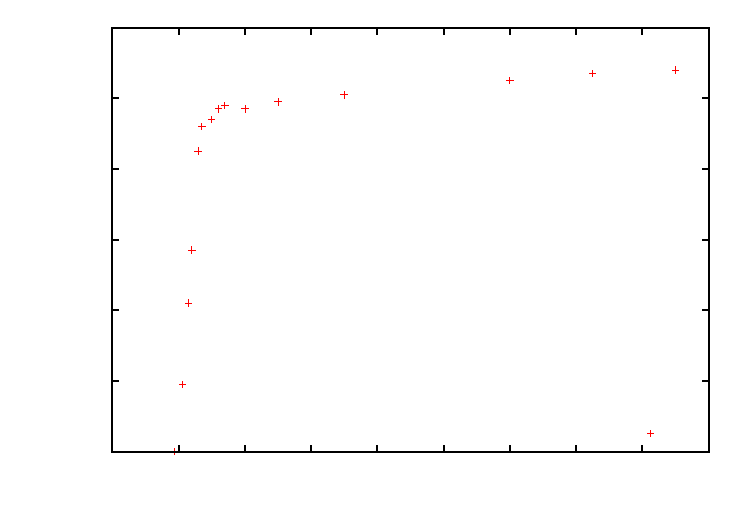
\includegraphics{heiz18}}%
    \gplfronttext
  \end{picture}%
\endgroup
\end{adjustbox}}
  \hfill
  \subfigure[$I_\text H=1.9\,$A\label{fig:heiz19}]
  {\begin{adjustbox}{width=0.48\linewidth}% GNUPLOT: LaTeX picture with Postscript
\begingroup
  \makeatletter
  \providecommand\color[2][]{%
    \GenericError{(gnuplot) \space\space\space\@spaces}{%
      Package color not loaded in conjunction with
      terminal option `colourtext'%
    }{See the gnuplot documentation for explanation.%
    }{Either use 'blacktext' in gnuplot or load the package
      color.sty in LaTeX.}%
    \renewcommand\color[2][]{}%
  }%
  \providecommand\includegraphics[2][]{%
    \GenericError{(gnuplot) \space\space\space\@spaces}{%
      Package graphicx or graphics not loaded%
    }{See the gnuplot documentation for explanation.%
    }{The gnuplot epslatex terminal needs graphicx.sty or graphics.sty.}%
    \renewcommand\includegraphics[2][]{}%
  }%
  \providecommand\rotatebox[2]{#2}%
  \@ifundefined{ifGPcolor}{%
    \newif\ifGPcolor
    \GPcolortrue
  }{}%
  \@ifundefined{ifGPblacktext}{%
    \newif\ifGPblacktext
    \GPblacktexttrue
  }{}%
  % define a \g@addto@macro without @ in the name:
  \let\gplgaddtomacro\g@addto@macro
  % define empty templates for all commands taking text:
  \gdef\gplbacktext{}%
  \gdef\gplfronttext{}%
  \makeatother
  \ifGPblacktext
    % no textcolor at all
    \def\colorrgb#1{}%
    \def\colorgray#1{}%
  \else
    % gray or color?
    \ifGPcolor
      \def\colorrgb#1{\color[rgb]{#1}}%
      \def\colorgray#1{\color[gray]{#1}}%
      \expandafter\def\csname LTw\endcsname{\color{white}}%
      \expandafter\def\csname LTb\endcsname{\color{black}}%
      \expandafter\def\csname LTa\endcsname{\color{black}}%
      \expandafter\def\csname LT0\endcsname{\color[rgb]{1,0,0}}%
      \expandafter\def\csname LT1\endcsname{\color[rgb]{0,1,0}}%
      \expandafter\def\csname LT2\endcsname{\color[rgb]{0,0,1}}%
      \expandafter\def\csname LT3\endcsname{\color[rgb]{1,0,1}}%
      \expandafter\def\csname LT4\endcsname{\color[rgb]{0,1,1}}%
      \expandafter\def\csname LT5\endcsname{\color[rgb]{1,1,0}}%
      \expandafter\def\csname LT6\endcsname{\color[rgb]{0,0,0}}%
      \expandafter\def\csname LT7\endcsname{\color[rgb]{1,0.3,0}}%
      \expandafter\def\csname LT8\endcsname{\color[rgb]{0.5,0.5,0.5}}%
    \else
      % gray
      \def\colorrgb#1{\color{black}}%
      \def\colorgray#1{\color[gray]{#1}}%
      \expandafter\def\csname LTw\endcsname{\color{white}}%
      \expandafter\def\csname LTb\endcsname{\color{black}}%
      \expandafter\def\csname LTa\endcsname{\color{black}}%
      \expandafter\def\csname LT0\endcsname{\color{black}}%
      \expandafter\def\csname LT1\endcsname{\color{black}}%
      \expandafter\def\csname LT2\endcsname{\color{black}}%
      \expandafter\def\csname LT3\endcsname{\color{black}}%
      \expandafter\def\csname LT4\endcsname{\color{black}}%
      \expandafter\def\csname LT5\endcsname{\color{black}}%
      \expandafter\def\csname LT6\endcsname{\color{black}}%
      \expandafter\def\csname LT7\endcsname{\color{black}}%
      \expandafter\def\csname LT8\endcsname{\color{black}}%
    \fi
  \fi
  \setlength{\unitlength}{0.0500bp}%
  \begin{picture}(7200.00,5040.00)%
    \gplgaddtomacro\gplbacktext{%
      \csname LTb\endcsname%
      \put(946,704){\makebox(0,0)[r]{\strut{} 0}}%
      \put(946,1518){\makebox(0,0)[r]{\strut{} 0.5}}%
      \put(946,2332){\makebox(0,0)[r]{\strut{} 1}}%
      \put(946,3147){\makebox(0,0)[r]{\strut{} 1.5}}%
      \put(946,3961){\makebox(0,0)[r]{\strut{} 2}}%
      \put(946,4775){\makebox(0,0)[r]{\strut{} 2.5}}%
      \put(1078,484){\makebox(0,0){\strut{}-20}}%
      \put(1714,484){\makebox(0,0){\strut{} 0}}%
      \put(2350,484){\makebox(0,0){\strut{} 20}}%
      \put(2986,484){\makebox(0,0){\strut{} 40}}%
      \put(3622,484){\makebox(0,0){\strut{} 60}}%
      \put(4259,484){\makebox(0,0){\strut{} 80}}%
      \put(4895,484){\makebox(0,0){\strut{} 100}}%
      \put(5531,484){\makebox(0,0){\strut{} 120}}%
      \put(6167,484){\makebox(0,0){\strut{} 140}}%
      \put(6803,484){\makebox(0,0){\strut{} 160}}%
      \put(176,2739){\rotatebox{-270}{\makebox(0,0){\strut{}Anodenstrom $I_\text A \; [A]$}}}%
      \put(3940,154){\makebox(0,0){\strut{}Spannung U $[V]$}}%
    }%
    \gplgaddtomacro\gplfronttext{%
      \csname LTb\endcsname%
      \put(5816,877){\makebox(0,0)[r]{\strut{}$I_\text{H}=1.9$A}}%
    }%
    \gplbacktext
    \put(0,0){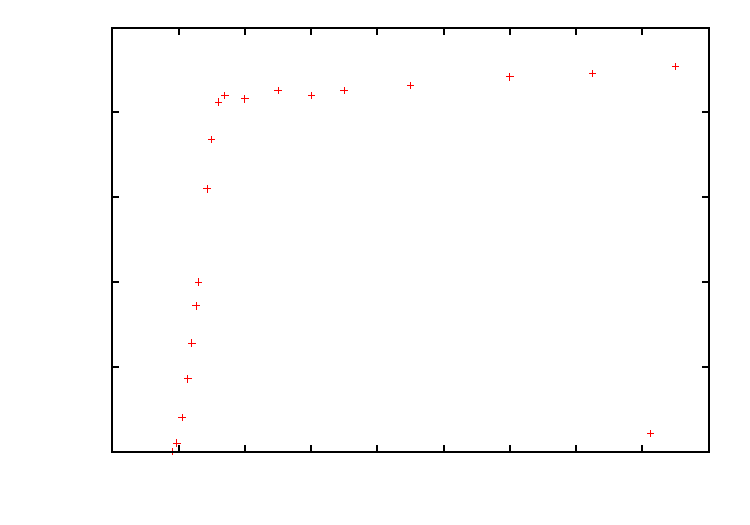
\includegraphics{heiz19}}%
    \gplfronttext
  \end{picture}%
\endgroup
\end{adjustbox}}
  \hfill
  \subfigure[$I_\text H=2.0\,$A\label{fig:heiz2}]
  {\begin{adjustbox}{width=0.48\linewidth}% GNUPLOT: LaTeX picture with Postscript
\begingroup
  \makeatletter
  \providecommand\color[2][]{%
    \GenericError{(gnuplot) \space\space\space\@spaces}{%
      Package color not loaded in conjunction with
      terminal option `colourtext'%
    }{See the gnuplot documentation for explanation.%
    }{Either use 'blacktext' in gnuplot or load the package
      color.sty in LaTeX.}%
    \renewcommand\color[2][]{}%
  }%
  \providecommand\includegraphics[2][]{%
    \GenericError{(gnuplot) \space\space\space\@spaces}{%
      Package graphicx or graphics not loaded%
    }{See the gnuplot documentation for explanation.%
    }{The gnuplot epslatex terminal needs graphicx.sty or graphics.sty.}%
    \renewcommand\includegraphics[2][]{}%
  }%
  \providecommand\rotatebox[2]{#2}%
  \@ifundefined{ifGPcolor}{%
    \newif\ifGPcolor
    \GPcolortrue
  }{}%
  \@ifundefined{ifGPblacktext}{%
    \newif\ifGPblacktext
    \GPblacktexttrue
  }{}%
  % define a \g@addto@macro without @ in the name:
  \let\gplgaddtomacro\g@addto@macro
  % define empty templates for all commands taking text:
  \gdef\gplbacktext{}%
  \gdef\gplfronttext{}%
  \makeatother
  \ifGPblacktext
    % no textcolor at all
    \def\colorrgb#1{}%
    \def\colorgray#1{}%
  \else
    % gray or color?
    \ifGPcolor
      \def\colorrgb#1{\color[rgb]{#1}}%
      \def\colorgray#1{\color[gray]{#1}}%
      \expandafter\def\csname LTw\endcsname{\color{white}}%
      \expandafter\def\csname LTb\endcsname{\color{black}}%
      \expandafter\def\csname LTa\endcsname{\color{black}}%
      \expandafter\def\csname LT0\endcsname{\color[rgb]{1,0,0}}%
      \expandafter\def\csname LT1\endcsname{\color[rgb]{0,1,0}}%
      \expandafter\def\csname LT2\endcsname{\color[rgb]{0,0,1}}%
      \expandafter\def\csname LT3\endcsname{\color[rgb]{1,0,1}}%
      \expandafter\def\csname LT4\endcsname{\color[rgb]{0,1,1}}%
      \expandafter\def\csname LT5\endcsname{\color[rgb]{1,1,0}}%
      \expandafter\def\csname LT6\endcsname{\color[rgb]{0,0,0}}%
      \expandafter\def\csname LT7\endcsname{\color[rgb]{1,0.3,0}}%
      \expandafter\def\csname LT8\endcsname{\color[rgb]{0.5,0.5,0.5}}%
    \else
      % gray
      \def\colorrgb#1{\color{black}}%
      \def\colorgray#1{\color[gray]{#1}}%
      \expandafter\def\csname LTw\endcsname{\color{white}}%
      \expandafter\def\csname LTb\endcsname{\color{black}}%
      \expandafter\def\csname LTa\endcsname{\color{black}}%
      \expandafter\def\csname LT0\endcsname{\color{black}}%
      \expandafter\def\csname LT1\endcsname{\color{black}}%
      \expandafter\def\csname LT2\endcsname{\color{black}}%
      \expandafter\def\csname LT3\endcsname{\color{black}}%
      \expandafter\def\csname LT4\endcsname{\color{black}}%
      \expandafter\def\csname LT5\endcsname{\color{black}}%
      \expandafter\def\csname LT6\endcsname{\color{black}}%
      \expandafter\def\csname LT7\endcsname{\color{black}}%
      \expandafter\def\csname LT8\endcsname{\color{black}}%
    \fi
  \fi
  \setlength{\unitlength}{0.0500bp}%
  \begin{picture}(7200.00,5040.00)%
    \gplgaddtomacro\gplbacktext{%
      \csname LTb\endcsname%
      \put(946,704){\makebox(0,0)[r]{\strut{} 0}}%
      \put(946,1111){\makebox(0,0)[r]{\strut{} 0.5}}%
      \put(946,1518){\makebox(0,0)[r]{\strut{} 1}}%
      \put(946,1925){\makebox(0,0)[r]{\strut{} 1.5}}%
      \put(946,2332){\makebox(0,0)[r]{\strut{} 2}}%
      \put(946,2740){\makebox(0,0)[r]{\strut{} 2.5}}%
      \put(946,3147){\makebox(0,0)[r]{\strut{} 3}}%
      \put(946,3554){\makebox(0,0)[r]{\strut{} 3.5}}%
      \put(946,3961){\makebox(0,0)[r]{\strut{} 4}}%
      \put(946,4368){\makebox(0,0)[r]{\strut{} 4.5}}%
      \put(946,4775){\makebox(0,0)[r]{\strut{} 5}}%
      \put(1078,484){\makebox(0,0){\strut{}-20}}%
      \put(1714,484){\makebox(0,0){\strut{} 0}}%
      \put(2350,484){\makebox(0,0){\strut{} 20}}%
      \put(2986,484){\makebox(0,0){\strut{} 40}}%
      \put(3622,484){\makebox(0,0){\strut{} 60}}%
      \put(4259,484){\makebox(0,0){\strut{} 80}}%
      \put(4895,484){\makebox(0,0){\strut{} 100}}%
      \put(5531,484){\makebox(0,0){\strut{} 120}}%
      \put(6167,484){\makebox(0,0){\strut{} 140}}%
      \put(6803,484){\makebox(0,0){\strut{} 160}}%
      \put(176,2739){\rotatebox{-270}{\makebox(0,0){\strut{}Anodenstrom $I_\text A \; [A]$}}}%
      \put(3940,154){\makebox(0,0){\strut{}Spannung U $[V]$}}%
    }%
    \gplgaddtomacro\gplfronttext{%
      \csname LTb\endcsname%
      \put(5816,877){\makebox(0,0)[r]{\strut{}$I_\text{H}=\SI{2.0}{\ampere}$}}%
    }%
    \gplbacktext
    \put(0,0){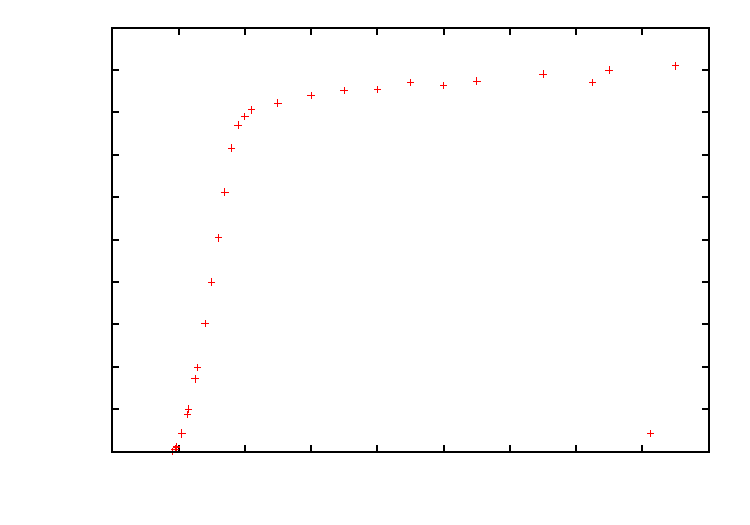
\includegraphics{heiz2}}%
    \gplfronttext
  \end{picture}%
\endgroup
\end{adjustbox}}
  \caption{Auftragung des Anodenstroms gegen die Anodenspannung bei verschiedenen Heizströmen}
  \label{fig:heiz}
\end{figure}
\begin{figure}[!h]
	\centering
	% GNUPLOT: LaTeX picture with Postscript
\begingroup
  \makeatletter
  \providecommand\color[2][]{%
    \GenericError{(gnuplot) \space\space\space\@spaces}{%
      Package color not loaded in conjunction with
      terminal option `colourtext'%
    }{See the gnuplot documentation for explanation.%
    }{Either use 'blacktext' in gnuplot or load the package
      color.sty in LaTeX.}%
    \renewcommand\color[2][]{}%
  }%
  \providecommand\includegraphics[2][]{%
    \GenericError{(gnuplot) \space\space\space\@spaces}{%
      Package graphicx or graphics not loaded%
    }{See the gnuplot documentation for explanation.%
    }{The gnuplot epslatex terminal needs graphicx.sty or graphics.sty.}%
    \renewcommand\includegraphics[2][]{}%
  }%
  \providecommand\rotatebox[2]{#2}%
  \@ifundefined{ifGPcolor}{%
    \newif\ifGPcolor
    \GPcolortrue
  }{}%
  \@ifundefined{ifGPblacktext}{%
    \newif\ifGPblacktext
    \GPblacktexttrue
  }{}%
  % define a \g@addto@macro without @ in the name:
  \let\gplgaddtomacro\g@addto@macro
  % define empty templates for all commands taking text:
  \gdef\gplbacktext{}%
  \gdef\gplfronttext{}%
  \makeatother
  \ifGPblacktext
    % no textcolor at all
    \def\colorrgb#1{}%
    \def\colorgray#1{}%
  \else
    % gray or color?
    \ifGPcolor
      \def\colorrgb#1{\color[rgb]{#1}}%
      \def\colorgray#1{\color[gray]{#1}}%
      \expandafter\def\csname LTw\endcsname{\color{white}}%
      \expandafter\def\csname LTb\endcsname{\color{black}}%
      \expandafter\def\csname LTa\endcsname{\color{black}}%
      \expandafter\def\csname LT0\endcsname{\color[rgb]{1,0,0}}%
      \expandafter\def\csname LT1\endcsname{\color[rgb]{0,1,0}}%
      \expandafter\def\csname LT2\endcsname{\color[rgb]{0,0,1}}%
      \expandafter\def\csname LT3\endcsname{\color[rgb]{1,0,1}}%
      \expandafter\def\csname LT4\endcsname{\color[rgb]{0,1,1}}%
      \expandafter\def\csname LT5\endcsname{\color[rgb]{1,1,0}}%
      \expandafter\def\csname LT6\endcsname{\color[rgb]{0,0,0}}%
      \expandafter\def\csname LT7\endcsname{\color[rgb]{1,0.3,0}}%
      \expandafter\def\csname LT8\endcsname{\color[rgb]{0.5,0.5,0.5}}%
    \else
      % gray
      \def\colorrgb#1{\color{black}}%
      \def\colorgray#1{\color[gray]{#1}}%
      \expandafter\def\csname LTw\endcsname{\color{white}}%
      \expandafter\def\csname LTb\endcsname{\color{black}}%
      \expandafter\def\csname LTa\endcsname{\color{black}}%
      \expandafter\def\csname LT0\endcsname{\color{black}}%
      \expandafter\def\csname LT1\endcsname{\color{black}}%
      \expandafter\def\csname LT2\endcsname{\color{black}}%
      \expandafter\def\csname LT3\endcsname{\color{black}}%
      \expandafter\def\csname LT4\endcsname{\color{black}}%
      \expandafter\def\csname LT5\endcsname{\color{black}}%
      \expandafter\def\csname LT6\endcsname{\color{black}}%
      \expandafter\def\csname LT7\endcsname{\color{black}}%
      \expandafter\def\csname LT8\endcsname{\color{black}}%
    \fi
  \fi
  \setlength{\unitlength}{0.0500bp}%
  \begin{picture}(7200.00,5040.00)%
    \gplgaddtomacro\gplbacktext{%
      \csname LTb\endcsname%
      \put(946,704){\makebox(0,0)[r]{\strut{} 0}}%
      \put(946,1111){\makebox(0,0)[r]{\strut{} 0.5}}%
      \put(946,1518){\makebox(0,0)[r]{\strut{} 1}}%
      \put(946,1925){\makebox(0,0)[r]{\strut{} 1.5}}%
      \put(946,2332){\makebox(0,0)[r]{\strut{} 2}}%
      \put(946,2740){\makebox(0,0)[r]{\strut{} 2.5}}%
      \put(946,3147){\makebox(0,0)[r]{\strut{} 3}}%
      \put(946,3554){\makebox(0,0)[r]{\strut{} 3.5}}%
      \put(946,3961){\makebox(0,0)[r]{\strut{} 4}}%
      \put(946,4368){\makebox(0,0)[r]{\strut{} 4.5}}%
      \put(946,4775){\makebox(0,0)[r]{\strut{} 5}}%
      \put(1078,484){\makebox(0,0){\strut{}-20}}%
      \put(1714,484){\makebox(0,0){\strut{} 0}}%
      \put(2350,484){\makebox(0,0){\strut{} 20}}%
      \put(2986,484){\makebox(0,0){\strut{} 40}}%
      \put(3622,484){\makebox(0,0){\strut{} 60}}%
      \put(4259,484){\makebox(0,0){\strut{} 80}}%
      \put(4895,484){\makebox(0,0){\strut{} 100}}%
      \put(5531,484){\makebox(0,0){\strut{} 120}}%
      \put(6167,484){\makebox(0,0){\strut{} 140}}%
      \put(6803,484){\makebox(0,0){\strut{} 160}}%
      \put(176,2739){\rotatebox{-270}{\makebox(0,0){\strut{}Anodenstrom $I_\text A \; [A]$}}}%
      \put(3940,154){\makebox(0,0){\strut{}Spannung U $[V]$}}%
    }%
    \gplgaddtomacro\gplfronttext{%
      \csname LTb\endcsname%
      \put(5816,4602){\makebox(0,0)[r]{\strut{}$I_\text{H}=2$A}}%
      \csname LTb\endcsname%
      \put(5816,4382){\makebox(0,0)[r]{\strut{}$I_\text{H}=1.9$A}}%
      \csname LTb\endcsname%
      \put(5816,4162){\makebox(0,0)[r]{\strut{}$I_\text{H}=1.8$A}}%
    }%
    \gplbacktext
    \put(0,0){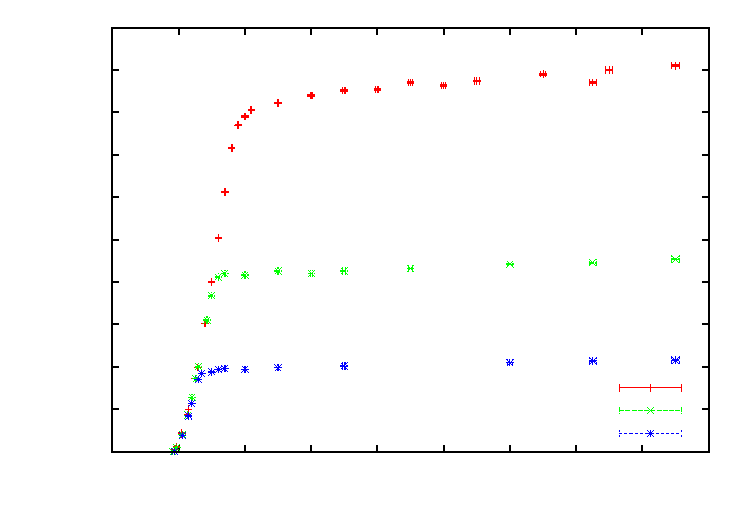
\includegraphics{heiz}}%
    \gplfronttext
  \end{picture}%
\endgroup

	\caption{Auftragung des Anodenstroms gegen die Anodenspannung bei unterschiedlichen Heizströmen}
	\label{fig:h}
\end{figure}


\subsection{Raumladung}
In Abbildung \ref{fig:raumladung} wird der Anodenstrom zur Potenz $\frac{2}{3}$ gegen die Anodenspannung aufgetragen.
Die Unterabbildungen zeigen hierbei die Daten für verschiedene Heizströme im Raumladungsgebiet.
Nach Formel \eqref{eq:rauml} ist ein linearer Zusammenhang hier zu erwarten.
Dieser gelt natürlich nur im Raumladungsgebiet, so dass auch nur dieser aufgetragen ist.

Die Gauß'sche Fehlerfortpflanzung liefert $\sigma_{I_A^{2/3}}=\frac{2\sigma_{a}}{3\sqrt[3]{a}}$.
Die Werte der linearen Regression sind in Tabelle \ref{tab:ParaRaum} zu finden.
Die ermittelten Werte haben eine Unsicherheit von höchstens $\sigma_a = 2.3\%$ und $\sigma_b=5.9\%$ und das reduzierte $\chi^2$ beträgt höchstens $0.2\%$.
Dies bedeutet, dass die Werte eine deutliche lineare Korrelation aufweisen.

Um die Kontaktspannung $U_K$ zu ermitteln, kann $0=a\cdot x + b$ umgestellt werden nach 
\begin{align*}
U_K &= -\frac{b}{a} \text{ mit}\\
\sigma_{U_K} &= \sqrt{\frac{\sigma_b^2}{a^2}+\frac{\sigma_a^2 \cdot b^2}{a^4}}\, .
\end{align*}
Die sich ergebenden Werte können ebenfalls in Tabelle \ref{tab:ParaRaum} entnommen werden.\\


\subsection{Exponent im Raumladungsbereich}
Nach Gl. \eqref{eq:rauml} ist für $I$ und $U_\text{ges}$ eine Relation
\begin{align}
I &= c\cdot U_\text{ges} = c\cdot \left( U_K+U_B \right)\\
\Rightarrow \ln (I) &= \ln c + \frac{2}{3} \ln \left( U_K + U_B \right)
\end{align}
für ein $c$ zu erwarten.

Wird nun $I$ gegen $U_\text{ges}$ doppelt logarithmisch aufgetragen, so sollte sich eine Geradensteigung von $m=\frac{2}{3}$ ergeben.
Die Fehlerrechnung nach Gauss führt zu
\begin{align}
\sigma_{\ln\left( U_K + U_B \right)}^2 &= \frac{\sigma_{U_K}^2 + \sigma_{U_B}^2}{U_K + U_B}\, \text{und}\\
\sigma_{\ln I} &= \frac{\sigma_I}{I}\,.
\end{align}

Dieser Plot ist in Abb. \ref{fig:expRauml} zu sehen und die gefitteten Parameter in Tabelle \ref{tab:expPara}.

\begin{figure}[h]
   \centering
   \subfigure[$I_\text A=1.8\,$A\label{fig:raum18}]
   {\begin{adjustbox}{width=0.48\linewidth}% GNUPLOT: LaTeX picture with Postscript
\begingroup
  \makeatletter
  \providecommand\color[2][]{%
    \GenericError{(gnuplot) \space\space\space\@spaces}{%
      Package color not loaded in conjunction with
      terminal option `colourtext'%
    }{See the gnuplot documentation for explanation.%
    }{Either use 'blacktext' in gnuplot or load the package
      color.sty in LaTeX.}%
    \renewcommand\color[2][]{}%
  }%
  \providecommand\includegraphics[2][]{%
    \GenericError{(gnuplot) \space\space\space\@spaces}{%
      Package graphicx or graphics not loaded%
    }{See the gnuplot documentation for explanation.%
    }{The gnuplot epslatex terminal needs graphicx.sty or graphics.sty.}%
    \renewcommand\includegraphics[2][]{}%
  }%
  \providecommand\rotatebox[2]{#2}%
  \@ifundefined{ifGPcolor}{%
    \newif\ifGPcolor
    \GPcolortrue
  }{}%
  \@ifundefined{ifGPblacktext}{%
    \newif\ifGPblacktext
    \GPblacktexttrue
  }{}%
  % define a \g@addto@macro without @ in the name:
  \let\gplgaddtomacro\g@addto@macro
  % define empty templates for all commands taking text:
  \gdef\gplbacktext{}%
  \gdef\gplfronttext{}%
  \makeatother
  \ifGPblacktext
    % no textcolor at all
    \def\colorrgb#1{}%
    \def\colorgray#1{}%
  \else
    % gray or color?
    \ifGPcolor
      \def\colorrgb#1{\color[rgb]{#1}}%
      \def\colorgray#1{\color[gray]{#1}}%
      \expandafter\def\csname LTw\endcsname{\color{white}}%
      \expandafter\def\csname LTb\endcsname{\color{black}}%
      \expandafter\def\csname LTa\endcsname{\color{black}}%
      \expandafter\def\csname LT0\endcsname{\color[rgb]{1,0,0}}%
      \expandafter\def\csname LT1\endcsname{\color[rgb]{0,1,0}}%
      \expandafter\def\csname LT2\endcsname{\color[rgb]{0,0,1}}%
      \expandafter\def\csname LT3\endcsname{\color[rgb]{1,0,1}}%
      \expandafter\def\csname LT4\endcsname{\color[rgb]{0,1,1}}%
      \expandafter\def\csname LT5\endcsname{\color[rgb]{1,1,0}}%
      \expandafter\def\csname LT6\endcsname{\color[rgb]{0,0,0}}%
      \expandafter\def\csname LT7\endcsname{\color[rgb]{1,0.3,0}}%
      \expandafter\def\csname LT8\endcsname{\color[rgb]{0.5,0.5,0.5}}%
    \else
      % gray
      \def\colorrgb#1{\color{black}}%
      \def\colorgray#1{\color[gray]{#1}}%
      \expandafter\def\csname LTw\endcsname{\color{white}}%
      \expandafter\def\csname LTb\endcsname{\color{black}}%
      \expandafter\def\csname LTa\endcsname{\color{black}}%
      \expandafter\def\csname LT0\endcsname{\color{black}}%
      \expandafter\def\csname LT1\endcsname{\color{black}}%
      \expandafter\def\csname LT2\endcsname{\color{black}}%
      \expandafter\def\csname LT3\endcsname{\color{black}}%
      \expandafter\def\csname LT4\endcsname{\color{black}}%
      \expandafter\def\csname LT5\endcsname{\color{black}}%
      \expandafter\def\csname LT6\endcsname{\color{black}}%
      \expandafter\def\csname LT7\endcsname{\color{black}}%
      \expandafter\def\csname LT8\endcsname{\color{black}}%
    \fi
  \fi
  \setlength{\unitlength}{0.0500bp}%
  \begin{picture}(7200.00,5040.00)%
    \gplgaddtomacro\gplbacktext{%
      \csname LTb\endcsname%
      \put(946,704){\makebox(0,0)[r]{\strut{} 0}}%
      \put(946,1111){\makebox(0,0)[r]{\strut{} 0.1}}%
      \put(946,1518){\makebox(0,0)[r]{\strut{} 0.2}}%
      \put(946,1925){\makebox(0,0)[r]{\strut{} 0.3}}%
      \put(946,2332){\makebox(0,0)[r]{\strut{} 0.4}}%
      \put(946,2740){\makebox(0,0)[r]{\strut{} 0.5}}%
      \put(946,3147){\makebox(0,0)[r]{\strut{} 0.6}}%
      \put(946,3554){\makebox(0,0)[r]{\strut{} 0.7}}%
      \put(946,3961){\makebox(0,0)[r]{\strut{} 0.8}}%
      \put(946,4368){\makebox(0,0)[r]{\strut{} 0.9}}%
      \put(946,4775){\makebox(0,0)[r]{\strut{} 1}}%
      \put(1078,484){\makebox(0,0){\strut{}-2}}%
      \put(1752,484){\makebox(0,0){\strut{}-1}}%
      \put(2425,484){\makebox(0,0){\strut{} 0}}%
      \put(3099,484){\makebox(0,0){\strut{} 1}}%
      \put(3772,484){\makebox(0,0){\strut{} 2}}%
      \put(4446,484){\makebox(0,0){\strut{} 3}}%
      \put(5119,484){\makebox(0,0){\strut{} 4}}%
      \put(5793,484){\makebox(0,0){\strut{} 5}}%
      \put(6466,484){\makebox(0,0){\strut{} 6}}%
      \put(176,2739){\rotatebox{-270}{\makebox(0,0){\strut{}Anodenstrom $\left(\frac{I_\text A}{1\,\text A}\right)^{2/3}$}}}%
      \put(3940,154){\makebox(0,0){\strut{}Spannung U $[V]$}}%
    }%
    \gplgaddtomacro\gplfronttext{%
      \csname LTb\endcsname%
      \put(5816,1097){\makebox(0,0)[r]{\strut{}$I_\text{H}=\SI{1.8}{\ampere}$}}%
      \csname LTb\endcsname%
      \put(5816,877){\makebox(0,0)[r]{\strut{}Lineare Regression}}%
    }%
    \gplbacktext
    \put(0,0){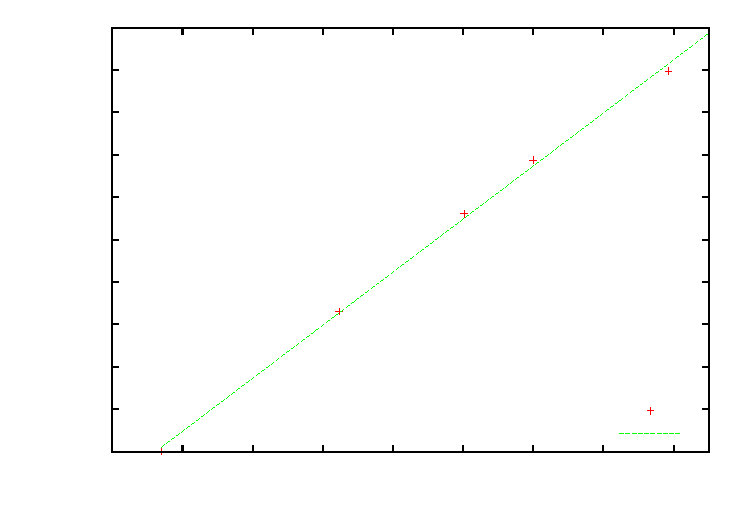
\includegraphics{raumladung18}}%
    \gplfronttext
  \end{picture}%
\endgroup
\end{adjustbox}}
   \hfill
   \subfigure[$I_\text A=1.9\,$A\label{fig:raum19}]
   {\begin{adjustbox}{width=0.48\linewidth}% GNUPLOT: LaTeX picture with Postscript
\begingroup
  \makeatletter
  \providecommand\color[2][]{%
    \GenericError{(gnuplot) \space\space\space\@spaces}{%
      Package color not loaded in conjunction with
      terminal option `colourtext'%
    }{See the gnuplot documentation for explanation.%
    }{Either use 'blacktext' in gnuplot or load the package
      color.sty in LaTeX.}%
    \renewcommand\color[2][]{}%
  }%
  \providecommand\includegraphics[2][]{%
    \GenericError{(gnuplot) \space\space\space\@spaces}{%
      Package graphicx or graphics not loaded%
    }{See the gnuplot documentation for explanation.%
    }{The gnuplot epslatex terminal needs graphicx.sty or graphics.sty.}%
    \renewcommand\includegraphics[2][]{}%
  }%
  \providecommand\rotatebox[2]{#2}%
  \@ifundefined{ifGPcolor}{%
    \newif\ifGPcolor
    \GPcolortrue
  }{}%
  \@ifundefined{ifGPblacktext}{%
    \newif\ifGPblacktext
    \GPblacktexttrue
  }{}%
  % define a \g@addto@macro without @ in the name:
  \let\gplgaddtomacro\g@addto@macro
  % define empty templates for all commands taking text:
  \gdef\gplbacktext{}%
  \gdef\gplfronttext{}%
  \makeatother
  \ifGPblacktext
    % no textcolor at all
    \def\colorrgb#1{}%
    \def\colorgray#1{}%
  \else
    % gray or color?
    \ifGPcolor
      \def\colorrgb#1{\color[rgb]{#1}}%
      \def\colorgray#1{\color[gray]{#1}}%
      \expandafter\def\csname LTw\endcsname{\color{white}}%
      \expandafter\def\csname LTb\endcsname{\color{black}}%
      \expandafter\def\csname LTa\endcsname{\color{black}}%
      \expandafter\def\csname LT0\endcsname{\color[rgb]{1,0,0}}%
      \expandafter\def\csname LT1\endcsname{\color[rgb]{0,1,0}}%
      \expandafter\def\csname LT2\endcsname{\color[rgb]{0,0,1}}%
      \expandafter\def\csname LT3\endcsname{\color[rgb]{1,0,1}}%
      \expandafter\def\csname LT4\endcsname{\color[rgb]{0,1,1}}%
      \expandafter\def\csname LT5\endcsname{\color[rgb]{1,1,0}}%
      \expandafter\def\csname LT6\endcsname{\color[rgb]{0,0,0}}%
      \expandafter\def\csname LT7\endcsname{\color[rgb]{1,0.3,0}}%
      \expandafter\def\csname LT8\endcsname{\color[rgb]{0.5,0.5,0.5}}%
    \else
      % gray
      \def\colorrgb#1{\color{black}}%
      \def\colorgray#1{\color[gray]{#1}}%
      \expandafter\def\csname LTw\endcsname{\color{white}}%
      \expandafter\def\csname LTb\endcsname{\color{black}}%
      \expandafter\def\csname LTa\endcsname{\color{black}}%
      \expandafter\def\csname LT0\endcsname{\color{black}}%
      \expandafter\def\csname LT1\endcsname{\color{black}}%
      \expandafter\def\csname LT2\endcsname{\color{black}}%
      \expandafter\def\csname LT3\endcsname{\color{black}}%
      \expandafter\def\csname LT4\endcsname{\color{black}}%
      \expandafter\def\csname LT5\endcsname{\color{black}}%
      \expandafter\def\csname LT6\endcsname{\color{black}}%
      \expandafter\def\csname LT7\endcsname{\color{black}}%
      \expandafter\def\csname LT8\endcsname{\color{black}}%
    \fi
  \fi
  \setlength{\unitlength}{0.0500bp}%
  \begin{picture}(7200.00,5040.00)%
    \gplgaddtomacro\gplbacktext{%
      \csname LTb\endcsname%
      \put(946,704){\makebox(0,0)[r]{\strut{}-0.2}}%
      \put(946,1156){\makebox(0,0)[r]{\strut{} 0}}%
      \put(946,1609){\makebox(0,0)[r]{\strut{} 0.2}}%
      \put(946,2061){\makebox(0,0)[r]{\strut{} 0.4}}%
      \put(946,2513){\makebox(0,0)[r]{\strut{} 0.6}}%
      \put(946,2966){\makebox(0,0)[r]{\strut{} 0.8}}%
      \put(946,3418){\makebox(0,0)[r]{\strut{} 1}}%
      \put(946,3870){\makebox(0,0)[r]{\strut{} 1.2}}%
      \put(946,4323){\makebox(0,0)[r]{\strut{} 1.4}}%
      \put(946,4775){\makebox(0,0)[r]{\strut{} 1.6}}%
      \put(1078,484){\makebox(0,0){\strut{}-2}}%
      \put(2032,484){\makebox(0,0){\strut{} 0}}%
      \put(2986,484){\makebox(0,0){\strut{} 2}}%
      \put(3941,484){\makebox(0,0){\strut{} 4}}%
      \put(4895,484){\makebox(0,0){\strut{} 6}}%
      \put(5849,484){\makebox(0,0){\strut{} 8}}%
      \put(6803,484){\makebox(0,0){\strut{} 10}}%
      \put(176,2739){\rotatebox{-270}{\makebox(0,0){\strut{}Anodenstrom $\left(\frac{I_\text A}{1\,\text A}\right)^{2/3}$}}}%
      \put(3940,154){\makebox(0,0){\strut{}Spannung U $[V]$}}%
    }%
    \gplgaddtomacro\gplfronttext{%
      \csname LTb\endcsname%
      \put(5816,1097){\makebox(0,0)[r]{\strut{}$I_\text{H}=\SI{1.9}{\ampere}$}}%
      \csname LTb\endcsname%
      \put(5816,877){\makebox(0,0)[r]{\strut{}Lineare Regression}}%
    }%
    \gplbacktext
    \put(0,0){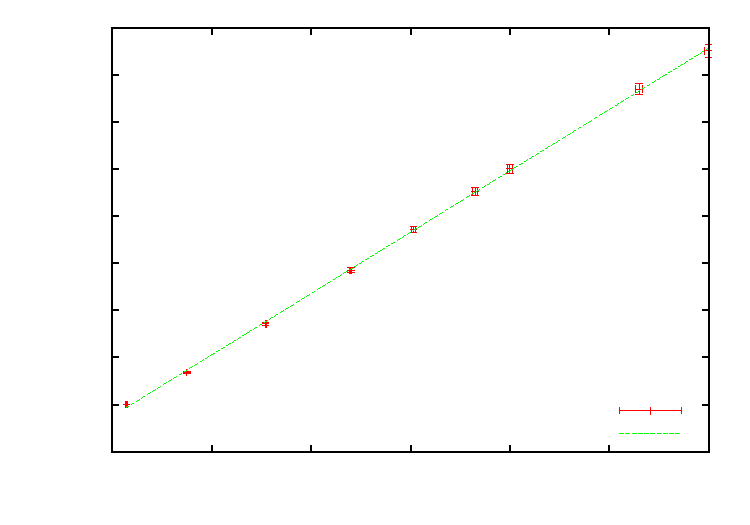
\includegraphics{raumladung19}}%
    \gplfronttext
  \end{picture}%
\endgroup
\end{adjustbox}}
   \hfill
   \subfigure[$I_\text A=2.0\,$A\label{fig:raum2}]
   {\begin{adjustbox}{width=0.48\linewidth}% GNUPLOT: LaTeX picture with Postscript
\begingroup
  \makeatletter
  \providecommand\color[2][]{%
    \GenericError{(gnuplot) \space\space\space\@spaces}{%
      Package color not loaded in conjunction with
      terminal option `colourtext'%
    }{See the gnuplot documentation for explanation.%
    }{Either use 'blacktext' in gnuplot or load the package
      color.sty in LaTeX.}%
    \renewcommand\color[2][]{}%
  }%
  \providecommand\includegraphics[2][]{%
    \GenericError{(gnuplot) \space\space\space\@spaces}{%
      Package graphicx or graphics not loaded%
    }{See the gnuplot documentation for explanation.%
    }{The gnuplot epslatex terminal needs graphicx.sty or graphics.sty.}%
    \renewcommand\includegraphics[2][]{}%
  }%
  \providecommand\rotatebox[2]{#2}%
  \@ifundefined{ifGPcolor}{%
    \newif\ifGPcolor
    \GPcolortrue
  }{}%
  \@ifundefined{ifGPblacktext}{%
    \newif\ifGPblacktext
    \GPblacktexttrue
  }{}%
  % define a \g@addto@macro without @ in the name:
  \let\gplgaddtomacro\g@addto@macro
  % define empty templates for all commands taking text:
  \gdef\gplbacktext{}%
  \gdef\gplfronttext{}%
  \makeatother
  \ifGPblacktext
    % no textcolor at all
    \def\colorrgb#1{}%
    \def\colorgray#1{}%
  \else
    % gray or color?
    \ifGPcolor
      \def\colorrgb#1{\color[rgb]{#1}}%
      \def\colorgray#1{\color[gray]{#1}}%
      \expandafter\def\csname LTw\endcsname{\color{white}}%
      \expandafter\def\csname LTb\endcsname{\color{black}}%
      \expandafter\def\csname LTa\endcsname{\color{black}}%
      \expandafter\def\csname LT0\endcsname{\color[rgb]{1,0,0}}%
      \expandafter\def\csname LT1\endcsname{\color[rgb]{0,1,0}}%
      \expandafter\def\csname LT2\endcsname{\color[rgb]{0,0,1}}%
      \expandafter\def\csname LT3\endcsname{\color[rgb]{1,0,1}}%
      \expandafter\def\csname LT4\endcsname{\color[rgb]{0,1,1}}%
      \expandafter\def\csname LT5\endcsname{\color[rgb]{1,1,0}}%
      \expandafter\def\csname LT6\endcsname{\color[rgb]{0,0,0}}%
      \expandafter\def\csname LT7\endcsname{\color[rgb]{1,0.3,0}}%
      \expandafter\def\csname LT8\endcsname{\color[rgb]{0.5,0.5,0.5}}%
    \else
      % gray
      \def\colorrgb#1{\color{black}}%
      \def\colorgray#1{\color[gray]{#1}}%
      \expandafter\def\csname LTw\endcsname{\color{white}}%
      \expandafter\def\csname LTb\endcsname{\color{black}}%
      \expandafter\def\csname LTa\endcsname{\color{black}}%
      \expandafter\def\csname LT0\endcsname{\color{black}}%
      \expandafter\def\csname LT1\endcsname{\color{black}}%
      \expandafter\def\csname LT2\endcsname{\color{black}}%
      \expandafter\def\csname LT3\endcsname{\color{black}}%
      \expandafter\def\csname LT4\endcsname{\color{black}}%
      \expandafter\def\csname LT5\endcsname{\color{black}}%
      \expandafter\def\csname LT6\endcsname{\color{black}}%
      \expandafter\def\csname LT7\endcsname{\color{black}}%
      \expandafter\def\csname LT8\endcsname{\color{black}}%
    \fi
  \fi
  \setlength{\unitlength}{0.0500bp}%
  \begin{picture}(7200.00,5040.00)%
    \gplgaddtomacro\gplbacktext{%
      \csname LTb\endcsname%
      \put(946,704){\makebox(0,0)[r]{\strut{} 0}}%
      \put(946,1383){\makebox(0,0)[r]{\strut{} 0.5}}%
      \put(946,2061){\makebox(0,0)[r]{\strut{} 1}}%
      \put(946,2740){\makebox(0,0)[r]{\strut{} 1.5}}%
      \put(946,3418){\makebox(0,0)[r]{\strut{} 2}}%
      \put(946,4097){\makebox(0,0)[r]{\strut{} 2.5}}%
      \put(946,4775){\makebox(0,0)[r]{\strut{} 3}}%
      \put(1078,484){\makebox(0,0){\strut{}-2}}%
      \put(1651,484){\makebox(0,0){\strut{} 0}}%
      \put(2223,484){\makebox(0,0){\strut{} 2}}%
      \put(2796,484){\makebox(0,0){\strut{} 4}}%
      \put(3368,484){\makebox(0,0){\strut{} 6}}%
      \put(3941,484){\makebox(0,0){\strut{} 8}}%
      \put(4513,484){\makebox(0,0){\strut{} 10}}%
      \put(5086,484){\makebox(0,0){\strut{} 12}}%
      \put(5658,484){\makebox(0,0){\strut{} 14}}%
      \put(6231,484){\makebox(0,0){\strut{} 16}}%
      \put(6803,484){\makebox(0,0){\strut{} 18}}%
      \put(176,2739){\rotatebox{-270}{\makebox(0,0){\strut{}Anodenstrom $\left(\frac{I_\text A}{1\,\text A}\right)^{2/3}$}}}%
      \put(3940,154){\makebox(0,0){\strut{}Spannung U $[V]$}}%
    }%
    \gplgaddtomacro\gplfronttext{%
      \csname LTb\endcsname%
      \put(5816,1097){\makebox(0,0)[r]{\strut{}$I_\text{H}=\SI{2.0}{\ampere}$}}%
      \csname LTb\endcsname%
      \put(5816,877){\makebox(0,0)[r]{\strut{}Lineare Regression}}%
    }%
    \gplbacktext
    \put(0,0){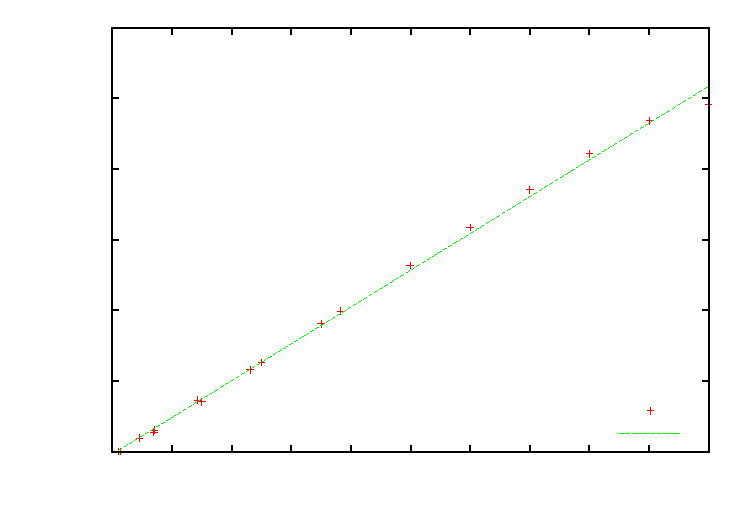
\includegraphics{raumladung2}}%
    \gplfronttext
  \end{picture}%
\endgroup
\end{adjustbox}}
   \caption{Auftragung des Anodenstroms zur Potenz $\frac{2}{3}$ gegen die Anodenspannung bei verchiedenen Heizströmen im Raumladungsgebiet.}
   \label{fig:raumladung}
 \end{figure}

\begin{table}[!h]
\centering
\begin{tabular}{|c|c|c|c|}
\hline
$I_\text H\,$[A]& $a\,\left[\frac{\text A^{2/3}}{\text V}\right]$	& $b\,\left[\text A^{2/3}\right]$ & $U_K \; [V]$	\\\hline\hline
1.8 		& $0.125\pm 0.003$	& $0.173\pm 0.011$		&$-1.38 \pm 0.09$	\\\hline
1.9 		& $0.1302\pm0.0009$ 	& $0.211\pm 0.005$		&$-1.62 \pm 0.04$	\\\hline
2.0 		& $0.1302\pm 0.0016$	& $0.242 \pm 0.014$		&$-1.9 \pm 0.1	$	\\\hline
\end{tabular}
\caption{Parameter aus den Linearen Regressionen von Abb. \ref{fig:raumladung} und die sich ergebende Kontaktspannung.}
\label{tab:ParaRaum}
\end{table}


\begin{figure}[!h]
\centering
% GNUPLOT: LaTeX picture with Postscript
\begingroup
  \makeatletter
  \providecommand\color[2][]{%
    \GenericError{(gnuplot) \space\space\space\@spaces}{%
      Package color not loaded in conjunction with
      terminal option `colourtext'%
    }{See the gnuplot documentation for explanation.%
    }{Either use 'blacktext' in gnuplot or load the package
      color.sty in LaTeX.}%
    \renewcommand\color[2][]{}%
  }%
  \providecommand\includegraphics[2][]{%
    \GenericError{(gnuplot) \space\space\space\@spaces}{%
      Package graphicx or graphics not loaded%
    }{See the gnuplot documentation for explanation.%
    }{The gnuplot epslatex terminal needs graphicx.sty or graphics.sty.}%
    \renewcommand\includegraphics[2][]{}%
  }%
  \providecommand\rotatebox[2]{#2}%
  \@ifundefined{ifGPcolor}{%
    \newif\ifGPcolor
    \GPcolortrue
  }{}%
  \@ifundefined{ifGPblacktext}{%
    \newif\ifGPblacktext
    \GPblacktexttrue
  }{}%
  % define a \g@addto@macro without @ in the name:
  \let\gplgaddtomacro\g@addto@macro
  % define empty templates for all commands taking text:
  \gdef\gplbacktext{}%
  \gdef\gplfronttext{}%
  \makeatother
  \ifGPblacktext
    % no textcolor at all
    \def\colorrgb#1{}%
    \def\colorgray#1{}%
  \else
    % gray or color?
    \ifGPcolor
      \def\colorrgb#1{\color[rgb]{#1}}%
      \def\colorgray#1{\color[gray]{#1}}%
      \expandafter\def\csname LTw\endcsname{\color{white}}%
      \expandafter\def\csname LTb\endcsname{\color{black}}%
      \expandafter\def\csname LTa\endcsname{\color{black}}%
      \expandafter\def\csname LT0\endcsname{\color[rgb]{1,0,0}}%
      \expandafter\def\csname LT1\endcsname{\color[rgb]{0,1,0}}%
      \expandafter\def\csname LT2\endcsname{\color[rgb]{0,0,1}}%
      \expandafter\def\csname LT3\endcsname{\color[rgb]{1,0,1}}%
      \expandafter\def\csname LT4\endcsname{\color[rgb]{0,1,1}}%
      \expandafter\def\csname LT5\endcsname{\color[rgb]{1,1,0}}%
      \expandafter\def\csname LT6\endcsname{\color[rgb]{0,0,0}}%
      \expandafter\def\csname LT7\endcsname{\color[rgb]{1,0.3,0}}%
      \expandafter\def\csname LT8\endcsname{\color[rgb]{0.5,0.5,0.5}}%
    \else
      % gray
      \def\colorrgb#1{\color{black}}%
      \def\colorgray#1{\color[gray]{#1}}%
      \expandafter\def\csname LTw\endcsname{\color{white}}%
      \expandafter\def\csname LTb\endcsname{\color{black}}%
      \expandafter\def\csname LTa\endcsname{\color{black}}%
      \expandafter\def\csname LT0\endcsname{\color{black}}%
      \expandafter\def\csname LT1\endcsname{\color{black}}%
      \expandafter\def\csname LT2\endcsname{\color{black}}%
      \expandafter\def\csname LT3\endcsname{\color{black}}%
      \expandafter\def\csname LT4\endcsname{\color{black}}%
      \expandafter\def\csname LT5\endcsname{\color{black}}%
      \expandafter\def\csname LT6\endcsname{\color{black}}%
      \expandafter\def\csname LT7\endcsname{\color{black}}%
      \expandafter\def\csname LT8\endcsname{\color{black}}%
    \fi
  \fi
  \setlength{\unitlength}{0.0500bp}%
  \begin{picture}(7200.00,5040.00)%
    \gplgaddtomacro\gplbacktext{%
      \csname LTb\endcsname%
      \put(1078,704){\makebox(0,0)[r]{\strut{}-10.5}}%
      \put(1078,1156){\makebox(0,0)[r]{\strut{}-10}}%
      \put(1078,1609){\makebox(0,0)[r]{\strut{}-9.5}}%
      \put(1078,2061){\makebox(0,0)[r]{\strut{}-9}}%
      \put(1078,2513){\makebox(0,0)[r]{\strut{}-8.5}}%
      \put(1078,2966){\makebox(0,0)[r]{\strut{}-8}}%
      \put(1078,3418){\makebox(0,0)[r]{\strut{}-7.5}}%
      \put(1078,3870){\makebox(0,0)[r]{\strut{}-7}}%
      \put(1078,4323){\makebox(0,0)[r]{\strut{}-6.5}}%
      \put(1078,4775){\makebox(0,0)[r]{\strut{}-6}}%
      \put(1210,484){\makebox(0,0){\strut{}-0.5}}%
      \put(2174,484){\makebox(0,0){\strut{} 0}}%
      \put(3139,484){\makebox(0,0){\strut{} 0.5}}%
      \put(4103,484){\makebox(0,0){\strut{} 1}}%
      \put(5067,484){\makebox(0,0){\strut{} 1.5}}%
      \put(6032,484){\makebox(0,0){\strut{} 2}}%
      \put(176,2739){\rotatebox{-270}{\makebox(0,0){\strut{}$\ln(I_\text A) \; [\ln(A))]$}}}%
      \put(4006,154){\makebox(0,0){\strut{}$\ln(U_\text{ges}) \; [\ln(V)]$}}%
    }%
    \gplgaddtomacro\gplfronttext{%
      \csname LTb\endcsname%
      \put(5816,1317){\makebox(0,0)[r]{\strut{}$I_\text{H}=\SI{1.8}{\ampere}$}}%
      \csname LTb\endcsname%
      \put(5816,1097){\makebox(0,0)[r]{\strut{}$I_\text{H}=\SI{1.9}{\ampere}$}}%
      \csname LTb\endcsname%
      \put(5816,877){\makebox(0,0)[r]{\strut{}$I_\text{H}=\SI{2}{\ampere}$}}%
    }%
    \gplbacktext
    \put(0,0){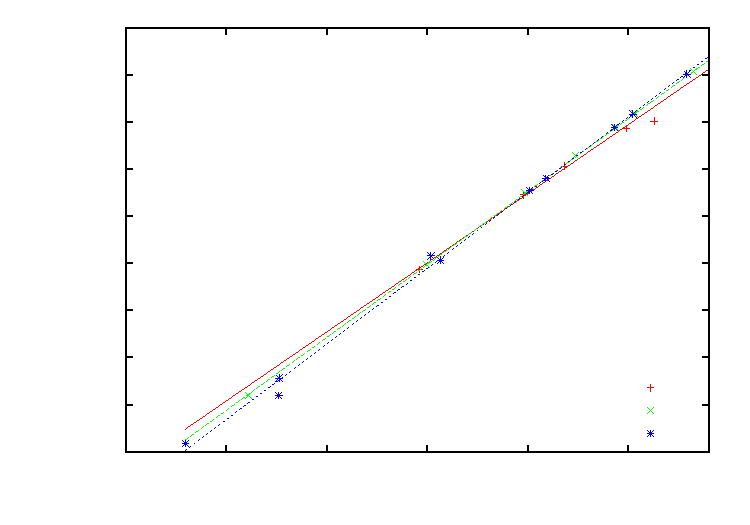
\includegraphics{exp}}%
    \gplfronttext
  \end{picture}%
\endgroup

\caption{Doppeltlogarithmische Auftragung von des Anodenstroms gegen die Gesamtspannung.}
\label{fig:expRauml}
\end{figure}

\begin{table}
\centering
\begin{tabular}{|c|c|}
\hline
$I_H\; [A]$	& Steigung $m\;[\ln\frac{A}{V}$\\\hline\hline
1.8	& $1.47 \pm 0.04$	\\\hline
1.9	& $1.547 \pm 0.009$	\\\hline
2	& $1.61 \pm 0.03$	\\\hline\hline
$\bar{m}$ & $1.549 \pm 0.008$\\\hline
\end{tabular}
\caption{gefitte Geradensteigung aus Abb. \ref{fig:expRauml}.}
\label{tab:expPara}
\end{table}

\section{Diskussion}
\label{sec:diskussion}
Das extra bereitstehende genauere analoge Amperemeter konnte leider auch die niedrigen Ströme nicht messen, da auch sie zu groß für das Gerät waren.
Auch bei der Messung des Anlaufstroms wirkte es nicht zuverlässig, da es über einen mehrere Volt großen Bereich keinen Strom anzeigte.
Daraufhin verwendeten wir nur die digitalen Messgeräte.

In Abb. \ref{fig:heiz} kann man erkennen, dass für die $2\,$A Messungen viele Messungen im Anlaufstrombereich gemacht wurden.
Für die $1.8\,$A Messung wurde dies kaum noch getan, so dass sich hier kaum Aussagen für diesen Bereich machen lassen.

Dennoch lassen die Werte aus Tabelle \ref{tab:ParaRaum} den Raumladungsbereich eingrenzen.
Für $1.8\,$A 


Die berechneten Werte der Kontaktspannung $U_K$ 

\bibliography{literatur}
\bibliographystyle{babalpha}
\end{document}
